\documentclass{beamer}
\usetheme[hideothersubsections]{PaloAlto}
\usecolortheme{albatross}

\usepackage{etoolbox}

\definecolor{Antra}{RGB}{105,105,105}
\definecolor{AntraB}{RGB}{105,105,125}
\definecolor{Gris}{RGB}{80,80,85}

\setbeamercolor*{structure}{fg=Antra!50,bg=AntraB}
\setbeamercolor*{palette primary}{use=structure,fg=white,bg=Gris}
\setbeamercolor*{background canvas}{bg=Antra,fg=Antra}
\setbeamercolor*{normal text}{bg=AntraB,fg=Antra!10}
\setbeamercolor*{navigation symbols}{bg=AntraB,fg=Antra!10}

\beamertemplatenavigationsymbolsempty


\title[Revue de projet Final]{Projet Aéroglisseur \\Revue de Projet Finale}
\author[]{Florian POUTHIER - Tristan DRUSSEL}
\date{Mai 2020}
\institute{4ème année Génie Électrique \\ INSA Strasbourg}

\setbeamertemplate{footline}
{
	\leavevmode% 
	\begin{beamercolorbox}[wd=0.3333\paperwidth,left,ht=0.025\paperheight,dp=0.0125\paperheight]{palette primary}
	   	\hspace*{2em}\insertauthor
	\end{beamercolorbox}
	\begin{beamercolorbox}[wd=0.3333\paperwidth,center,ht=0.025\paperheight,dp=0.0125\paperheight]{AntraB}
		\hspace*{2em} \textbf{\insertframenumber} \hspace*{2em}
	\end{beamercolorbox}
	\begin{beamercolorbox}[wd=0.3333\paperwidth,right,ht=0.025\paperheight,dp=0.0125\paperheight]{palette primary}
		\insertshorttitle\hspace*{2em}
	\end{beamercolorbox}
	\vskip0pt
}
\setbeamertemplate{caption}[numbered]

\begin{document}
	\begin{frame}[noframenumbering,plain]
		\titlepage
	\end{frame}
	\author[]{Tristan DRUSSEL}
	\begin{frame}
		\frametitle{Aperçu}
	%Contexte du projet
	%organisation du travail,problématique, questionnement reformulation du rpbleme
		\begin{columns}[T]
	  		\begin{column}{0.5\textwidth}
	  		\begin{itemize}
	  			\item Réalisation d'un aéroglisseur sur la base du Chticat
				\item Mise en oeuvre de l'électronique de puissance, de l'électronique numérique et de la mécanique
	  		\end{itemize}
	    	
	  		\end{column}
	  		\begin{column}{0.5\textwidth}
	  			\begin{figure}
	    			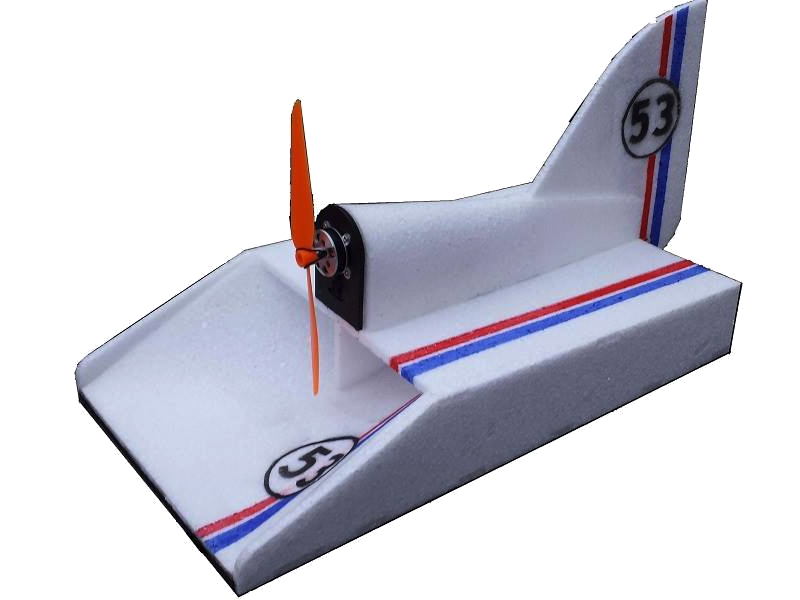
\includegraphics[width=0.8\textwidth]{../Illus/Chticat.png}
	    			\caption{Photo d'un Chticat originel}
	    		 \end{figure}
	  		\end{column}
		\end{columns}
	\end{frame}
	\begin{frame}{Sommaire}
	%Plan d'intervention succinct
		\setcounter{tocdepth}{1}
		\tableofcontents
	\end{frame}
	\begin{frame}{L'aspect mécanique}
		\section[Mécanique]{L'aspect Mécanique}
		\subsection{Modèle CAO}
		\begin{columns}[T]
	  		\begin{column}{0.5\textwidth}
		    	\begin{itemize}
		    		\item Récupération des sources
		    		\item Adaptation du modèle
		    	\end{itemize}
	  		\end{column}
	  		\begin{column}{0.5\textwidth}
	    		\begin{figure}
	    			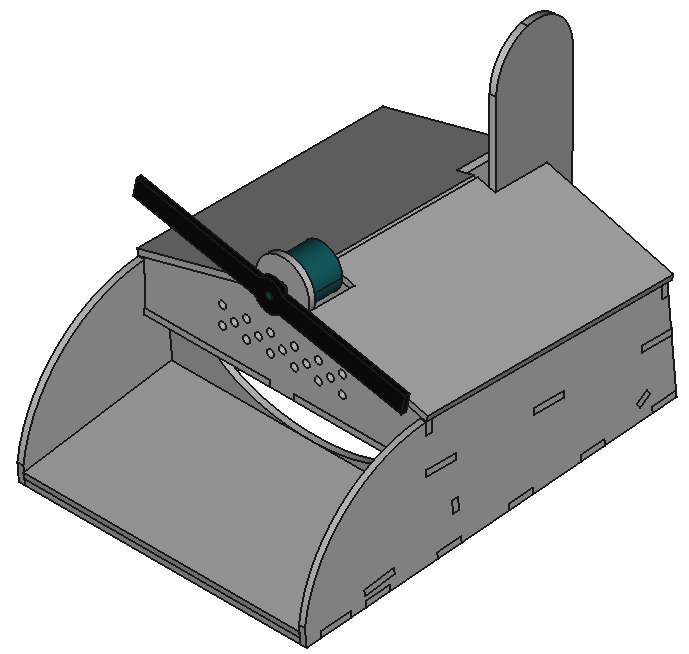
\includegraphics[width=0.8\textwidth]{../Illus/3dview.png}
	    			\caption{Modèle 3D modifié et adapté}
	    		 \end{figure}
	  		\end{column}
		\end{columns}
		
	\end{frame}
	\begin{frame}{Électronique Numérique}
		\section[ENUM]{L'aspect Électronique Numérique}
		Communication entre différents éléments:
		\begin{itemize}
			\item Application mobile
	  		\item Module Bluetooth: \texttt{HC-05}
			\item \texttt{PIC16F1619}
			\item \texttt{dsPIC10F2030}
	  	\end{itemize}
	  	Contrôle de l'onduleur
	\end{frame}
	\begin{frame}{Électronique Numérique:}
		\framesubtitle{Communication Bluetooth}
		\subsection[Bluetooth]{Communication Bluetooth}
		\begin{columns}[T]
	  		\begin{column}{0.5\textwidth}
		    	\begin{itemize}
		    		\item Contrôle à partir du Smartphone
		    	\end{itemize}
		    	\begin{figure}
		    		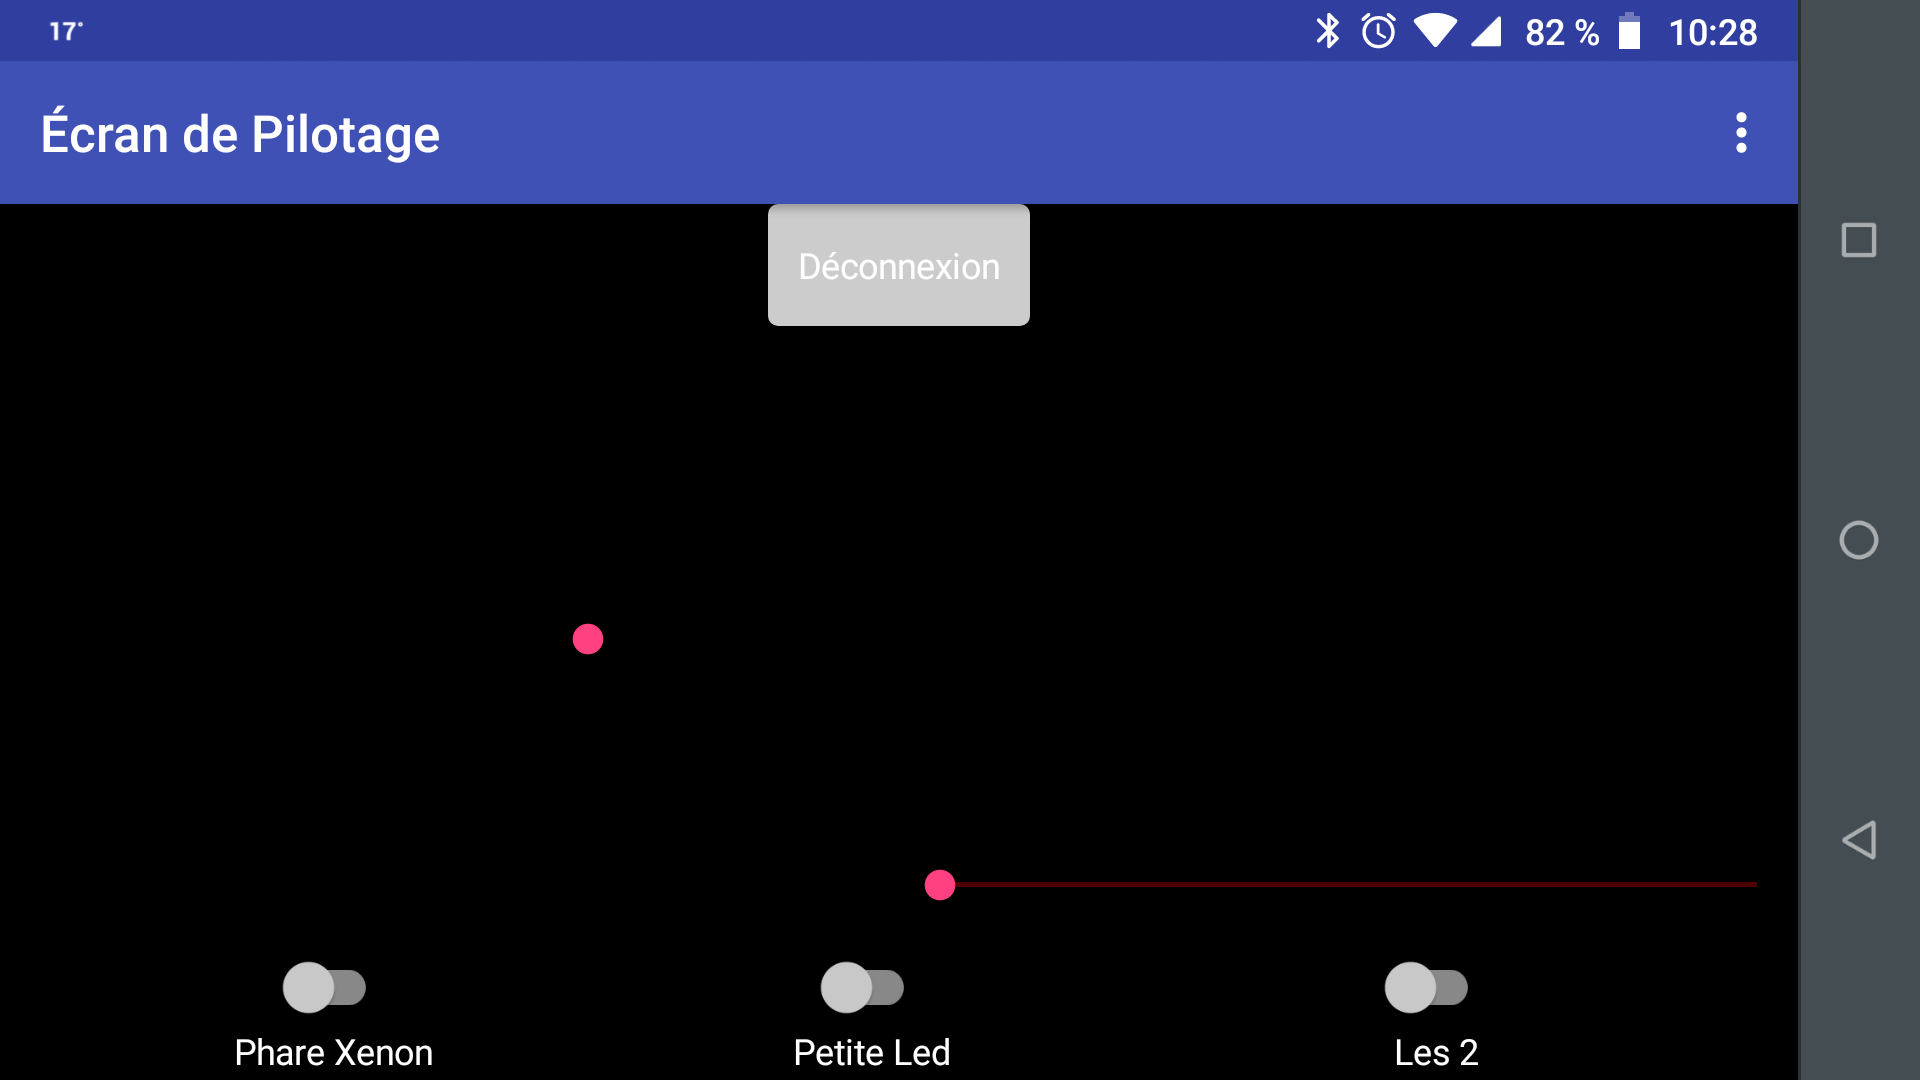
\includegraphics[width=0.8\textwidth]{../Illus/AppPilotage.png}
	    			\caption{Écran de pilotage de l'application}
	    		 \end{figure}
	  		\end{column}
	  		\begin{column}{0.5\textwidth}
	  			\begin{figure}
	    			\hspace*{2em}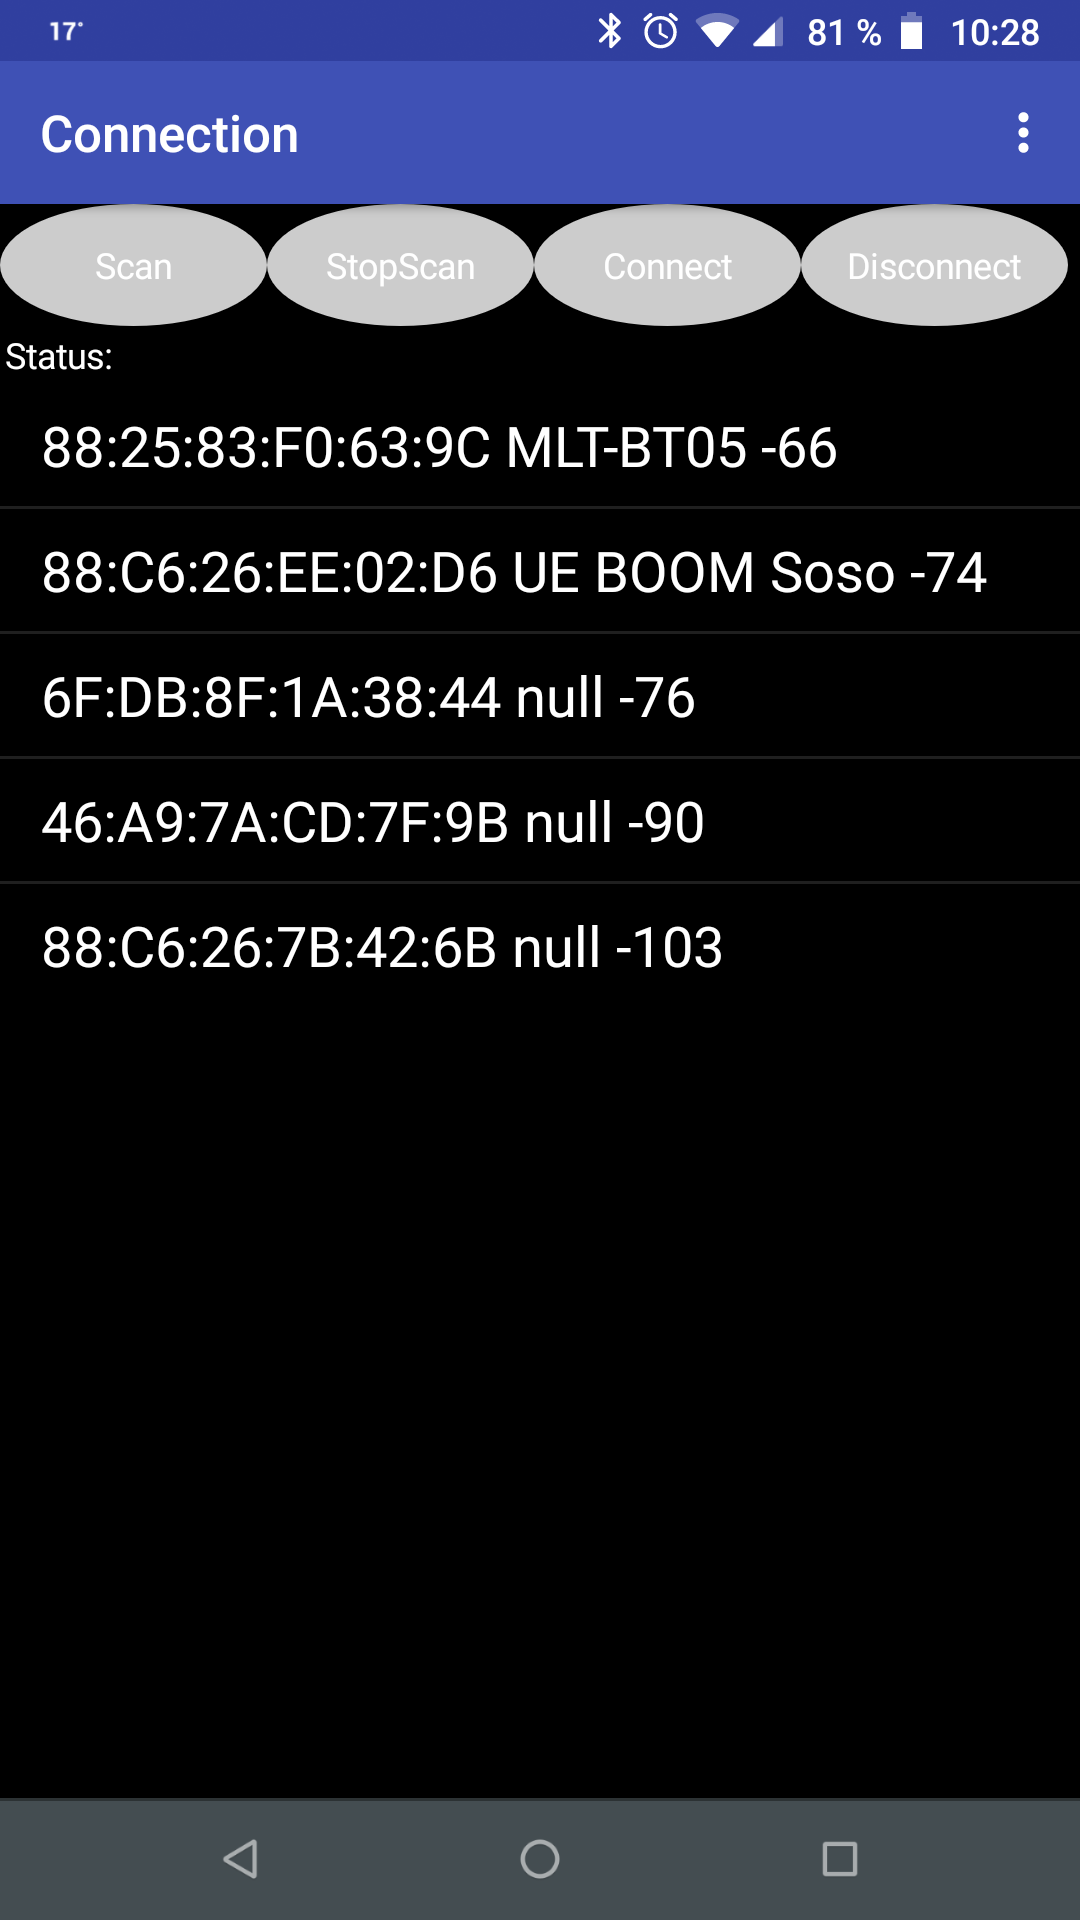
\includegraphics[height=0.8\textheight]{../Illus/AppConnection.png}
	    			\caption{Écran de connection de l'application}
	    		\end{figure}
	  		\end{column}
		\end{columns}
		
	\end{frame}
	\begin{frame}{Électronique Numérique:}
		\framesubtitle{Communication Série}
		\subsection[Série]{Communication Série}
		\begin{itemize}
		    \item Communication entre le Récepteur Bluetooth et le \texttt{PIC16F1619}
		\end{itemize}
		\begin{columns}[T]
	  		\begin{column}{0.5\textwidth}
		    	\begin{figure}
		    		
\includegraphics[width=0.45\textwidth]{../Illus/BluetoothLogo.png}
	    			\caption{Logo du Bluetooth}
	    		 \end{figure}
	  		\end{column}
	  		\begin{column}{0.5\textwidth}
	  			\begin{figure}
	    			\hspace*{2em}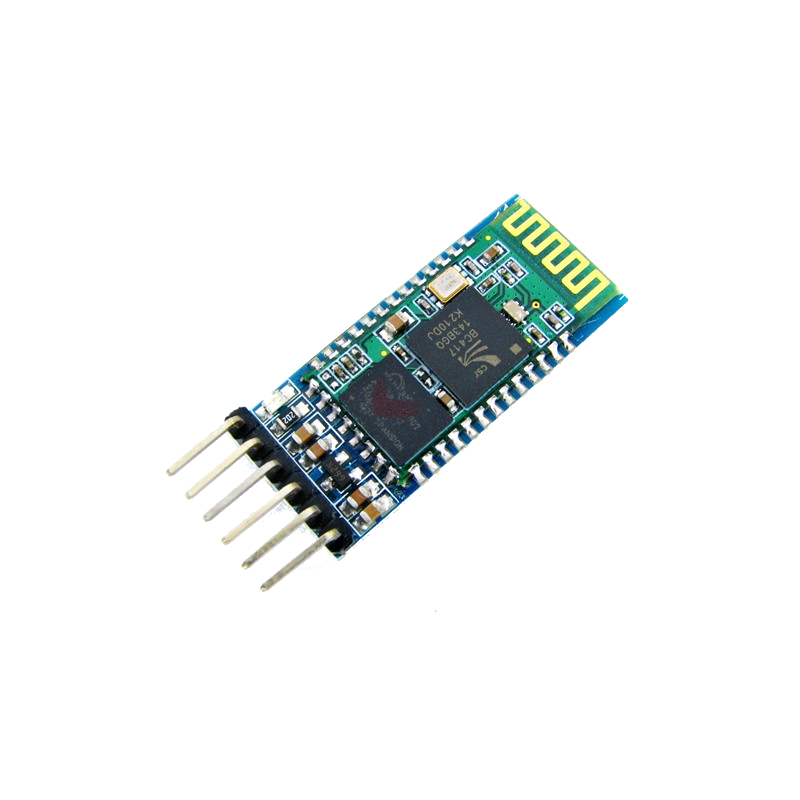
\includegraphics[width=0.7\textwidth]{../Illus/HC05.png}
	    			\caption{Module Bluetooth \texttt{HC-05}}
	    		\end{figure}
	  		\end{column}
	  	\end{columns}
	\end{frame}
	\begin{frame}{Électronique Numérique:}
	\framesubtitle{Communication \textit{Serial Peripheral Interface}}
		\subsection[SPI]{Communication SPI}
		\begin{itemize}
		    \item Communication entre le \texttt{PIC16F1619} et le \texttt{dsPIC10F2030}
		\end{itemize}
	\end{frame}
	
	\author[]{Florian POUTHIER}
	%Intro Power Electronics
	\begin{frame}{Power Electronics}
		\section[ENPU]{Power Electronics part}
		Power supply managing and three-phase inverter implementation
 		\begin{itemize}
			\item Functional analysis
			\item \textit{PSIM} simulations
			\item PCB designs
		\end{itemize}
	\end{frame}
	
	% Analyse fonctionnelle
	\begin{frame}{Power Electronics:}
		\framesubtitle{Functional analysis}
		\subsection[Func analysis]{Functional analysis}
		\begin{columns}[T]
	  		\begin{column}{0.4\textwidth}
				\begin{itemize}
					\item \textit{Brushless} motor internal structure
					\item Magnetic laws governing motor's motion settling
					\item Electronic circuit allowing motor control
				\end{itemize}
	  		\end{column}
	  		\begin{column}{0.6\textwidth}
	  			\vspace{-1em}
	  			\begin{figure}
	  				\begin{center}
	  					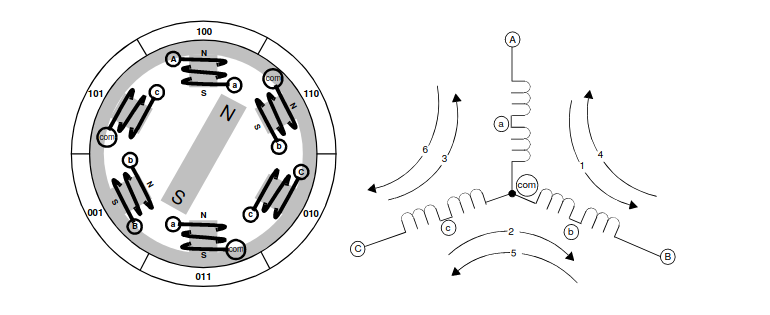
\includegraphics[height=0.3\textheight]{../Illus/struct_bldcm.png}
	  				\end{center}
	    			\caption{\textit{Brushless motor} structure and modelisation}
	    		\end{figure}
	    		\vspace{-2em}
	  			\begin{figure}
	  				\begin{center}
	  					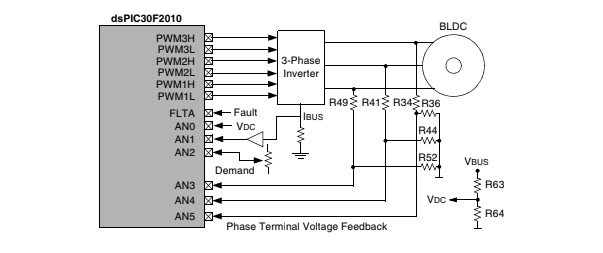
\includegraphics[height=0.3\textheight]{../Illus/back_emf_scheme.png}
	  				\end{center}
	    			\caption{Inverter and back electromagnetic force detection}
	    		\end{figure}
	  		\end{column}
		\end{columns}

	\end{frame}	
		
	% PSIM Simulations - Supply
	\begin{frame}{Power Electronics:}
		\framesubtitle{PSIM simulations}
		\subsection[Simulations]{PSIM simulations}
		\begin{columns}[T]
	  		\begin{column}{0.5\textwidth}
				Simulation of the power supply operation 
				\begin{itemize}
					\item Implementation of the \textit{Buck} based component's internal block diagram
					\item External components definition
					\item Model and external components' values validation
				\end{itemize}
	  		\end{column}
	  		\begin{column}{0.5\textwidth}
	  			\begin{figure}
	  				\begin{center}
	  					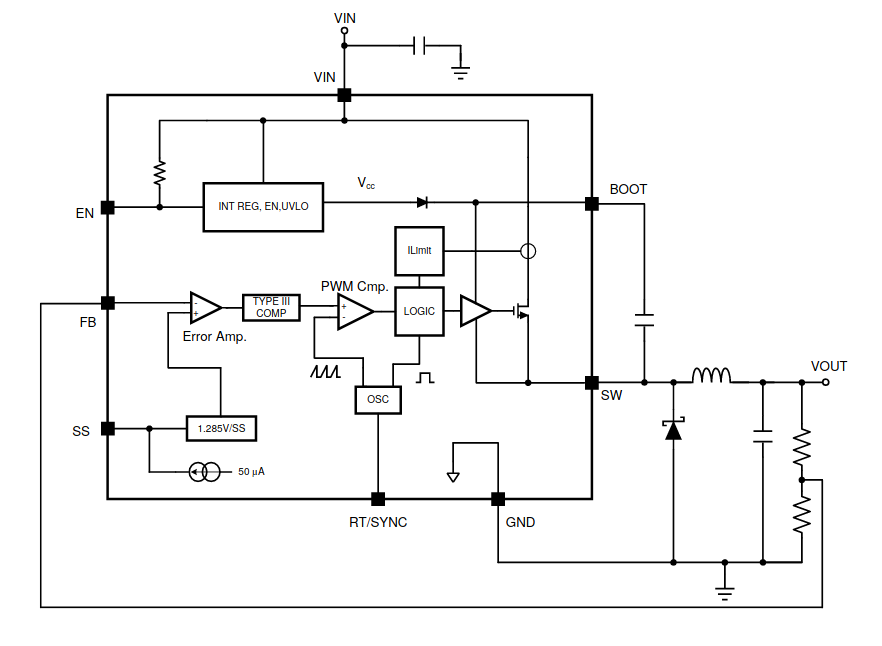
\includegraphics[height=0.5\textheight]{../Illus/func_bloc_lm22672.png}
	  				\end{center}
	    			\caption{LM22672 component's internal block diagram}
	    		\end{figure}
	  		\end{column}
		\end{columns}
	\end{frame}
	
	% PSIM simulations - BLDCM
	\begin{frame}{Power Electronics:}
		\framesubtitle{PSIM simulations}
		\begin{columns}[T]
	  		\begin{column}{0.5\textwidth}
				Simulation of the \textit{brushless} motor operation
				\begin{itemize}
					\item Study of the \textit{brushless} motor steering
					\item Mechanical aspects taken into account with propeller's mathematical modelisation
					\item Hoped propulsion performances verification
				\end{itemize}
	  		\end{column}
	  		\begin{column}{0.5\textwidth}
	  			\begin{figure}
	  				\begin{center}
	  					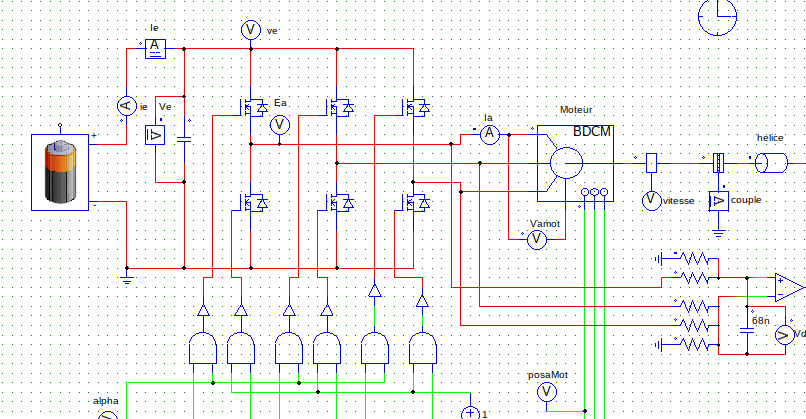
\includegraphics[height=0.35\textheight]{../Illus/simu_bldcm.png}
	  				\end{center}
	    			\caption{\textit{PSIM} implementation of the inverter and \textit{brushless} motor}
	    		\end{figure}
	  		\end{column}
		\end{columns}
	\end{frame}	
	
	% PCB Design - Supply PCB
	\begin{frame}{Power Electronics:}
		\framesubtitle{PCB Design}
		\subsection[PCB Design]{PCB Design}
		\begin{columns}[T]
	  		\begin{column}{0.5\textwidth}
	  			Power supply inteface
		    	\begin{itemize}
		    		\item Obtaining all main voltages required for system operation
		    		\item Electrical ground routed to avoid inrush current
		    		\item Component placement optimization to avoid electromagnetic compatibility
		    	\end{itemize}
	  		\end{column}
	  		\begin{column}{0.5\textwidth}
	  			\begin{figure}
	  				\begin{center}
	  					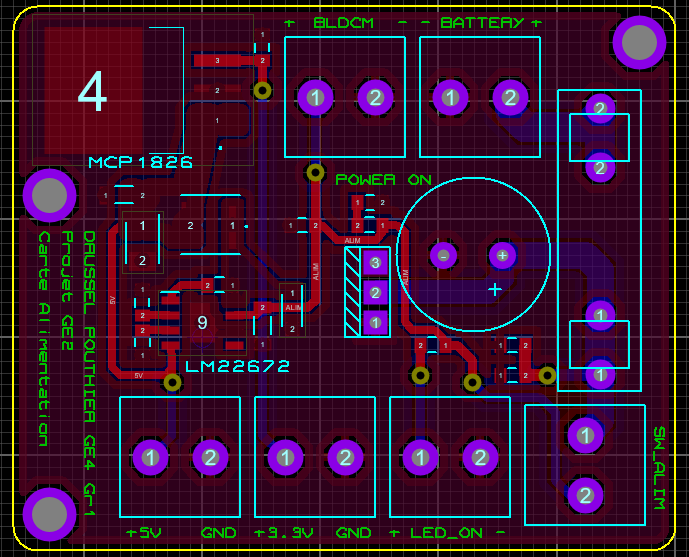
\includegraphics[height=0.5\textheight]{../Illus/PCB_Alim.PNG}
	  				\end{center}
	    			\caption{Power supply PCB view}
	    		\end{figure}
	  		\end{column}
		\end{columns}
	\end{frame}

	% PCB Design - One phase inverter PCB
	\begin{frame}{Power Electronics:}
		\framesubtitle{PCB Design}
		\begin{columns}[T]
	  		\begin{column}{0.6\textwidth}
	  			One phase inverter PCB
		    	\begin{itemize}
		    		\item Heat exchange surfaces determination according to MOSFET losses
		    		\item Use of MOSFET driver to interface PWM control and MOSFET switching
		    		\item Use of decoupling capacitor to avoid inrush currents throw power supply
		    	\end{itemize}
	  		\end{column}
	  		\begin{column}{0.4\textwidth}
	  			\begin{figure}
	  				\begin{center}
	  					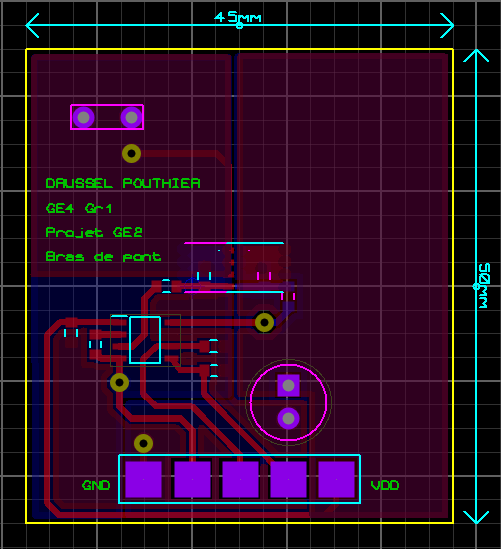
\includegraphics[height=0.5\textheight]{../Illus/PCB_Bras_de_pont.PNG}
	  				\end{center}
	    			\caption{One phase inverter PCB view}
	    		\end{figure}
	  		\end{column}
		\end{columns}
	\end{frame}
	
	% Conception des PCBs - Carte commande
	\begin{frame}{Power Electronics:}
		\framesubtitle{PCB Design}
		\begin{columns}[T]
	  		\begin{column}{0.5\textwidth}
	  			Main control PCB
		    	\begin{itemize}
		    		\item PIC microcontroller operation
		    		\item Managing user input informations received by Bluetooth communication
		    		\item Three phase inverter and servomotor control according to this input informations
		    	\end{itemize}
	  		\end{column}
	  		\begin{column}{0.5\textwidth}
	  			\begin{figure}
	  				\begin{center}
	  					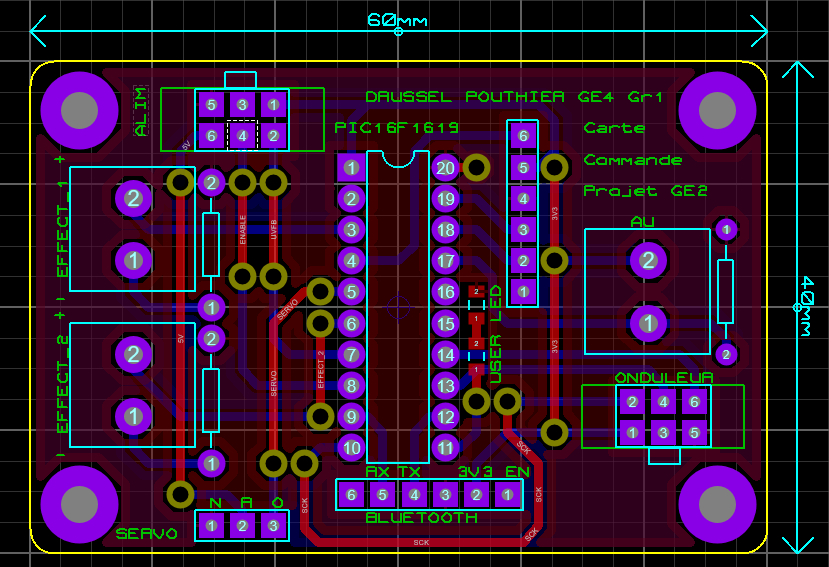
\includegraphics[height=0.4\textheight]{../Illus/PCB_Main.PNG}
	  				\end{center}
	    			\caption{Main control PCB view}
	    		\end{figure}
	  		\end{column}
		\end{columns}
	\end{frame}
	
	\begin{frame}{Pursuites du projet}
		\section[Poursuites]{Poursuites du projet}
		\begin{itemize}
		    \item Pilotage de l'onduleur
		    \item Réalisation des cartes	
		    \item Tests en conditions réelles
		\end{itemize}
	\end{frame}
	
	\begin{frame}{Conclusion}
	\section*{Conclusion}
	%Conclusion
	\begin{itemize}
		    \item Projet pluridisciplinaire
		    \item Mise en oeuvre des compétences acquises précédemment
		\end{itemize}
	\end{frame}
	\author[]{Florian POUTHIER - Tristan DRUSSEL}
	\begin{frame}[plain]{Merci de votre attention}
	\section*{}
		%remerciement
		\titlepage
	\end{frame}
\end{document}